% ============================================================================
% AI-Driven Positional Trading Strategy — NSE 100 Stocks
% Master's Thesis Presentation - Beamer LaTeX
% ============================================================================
\documentclass[aspectratio=43,11pt]{beamer}

% ================== THEME AND COLORS ==================
\usetheme{Madrid}
\usecolortheme{whale}

\definecolor{primaryblue}{RGB}{0,51,102}
\definecolor{accentorange}{RGB}{255,128,0}
\definecolor{lightgray}{RGB}{240,240,240}
\definecolor{successgreen}{RGB}{40,167,69}
\definecolor{warningred}{RGB}{220,53,69}

\setbeamercolor{palette primary}{bg=primaryblue,fg=white}
\setbeamercolor{palette secondary}{bg=primaryblue!80,fg=white}
\setbeamercolor{palette tertiary}{bg=primaryblue!60,fg=white}
\setbeamercolor{structure}{fg=primaryblue}
\setbeamercolor{title}{fg=white,bg=primaryblue}
\setbeamercolor{frametitle}{fg=white,bg=primaryblue}
\setbeamercolor{block title}{bg=primaryblue,fg=white}
\setbeamercolor{block body}{bg=lightgray}
\setbeamercolor{block title example}{bg=successgreen,fg=white}
\setbeamercolor{block title alerted}{bg=warningred,fg=white}

% ================== PACKAGES ==================
\usepackage{graphicx}
\usepackage{booktabs}
\usepackage{tabularx}
\usepackage{adjustbox}
\usepackage{amsmath,amssymb}
\usepackage{tikz}
\usepackage{multirow}
\usepackage{hyperref}
\hypersetup{pdfpagemode=UseNone,pdfpagelayout=OneColumn}
\usepackage{xcolor}
\usepackage{colortbl}
\usepackage{setspace}

\usetikzlibrary{shapes,arrows,positioning,calc,fit,backgrounds}

% ================== GLOBAL SETTINGS ==================
\setbeamertemplate{navigation symbols}{}
\setbeamertemplate{footline}[frame number]
\setbeamertemplate{itemize items}[circle]
\setbeamertemplate{enumerate items}[default]
% Tighten item spacing globally
\setlength{\leftmargini}{1.2em}
\setlength{\itemsep}{0pt}
\setlength{\parskip}{0pt}

\graphicspath{{../Master_thesis/images/}}

% Consistent small font for block content
\setbeamerfont{block body}{size=\footnotesize}
\setbeamerfont{block body example}{size=\footnotesize}
\setbeamerfont{block body alerted}{size=\footnotesize}

% ================== TITLE INFO ==================
\title[AI-Driven Positional Trading --- NSE]{\small\textbf{Development of Positional Trading Strategy Using Deep Learning and Its Training, Testing, and Implementation on a Real-Time Platform Using API}}
\subtitle{End Semester Project --- Phase 2 Presentation}
\author{Presented by: Vishwam Shah\\[0.15cm]
\small Under the Guidance of: Dr.~Jigarkumar Shah}
\institute{Pandit Deendayal Energy University \\ School of Technology}
\date{March 2026}
\titlegraphic{
\includegraphics[height=1.2cm]{pdeulogo.png}}

% ============================================================================
\begin{document}

% ================== TITLE SLIDE ==================
\begin{frame}
    \titlepage
\end{frame}

% ================== OUTLINE ==================
\begin{frame}{Presentation Outline}
    \tableofcontents
\end{frame}

% ============================================================================
\section{Introduction \& Motivation}
% ============================================================================

\begin{frame}{Research Motivation}
    \begin{columns}[T]
        \begin{column}{0.48\textwidth}
            \textbf{The Challenge:}
            \begin{itemize}\footnotesize\setlength{\itemsep}{3pt}
                \item NSE markets are volatile, non-linear, and regime-dependent
                \item Prior work used limited models and feature sets
                \item Phase~1 achieved 68\% accuracy --- later found to be inflated due to \textbf{data leakage}
                \item After fixing leakage, rigorous evaluation reveals true predictability
            \end{itemize}
            \vspace{0.2cm}
            \begin{alertblock}{Data Leakage Found \& Fixed}
                \footnotesize Phase~1 issues: scaler fitted on full dataset; global cues not time-shifted. \textbf{Fixed:} scaler fitted per train window only; all external cues shifted +1 day.
            \end{alertblock}
        \end{column}
        \begin{column}{0.48\textwidth}
            \begin{block}{Research Scope}
                \footnotesize\setlength{\itemsep}{2pt}
                \begin{itemize}
                    \item \textbf{100} NSE Nifty-100 Stocks
                    \item \textbf{$\sim$219} Raw Engineered Features
                    \item \textbf{50} Features after Selection
                    \item \textbf{10} Heterogeneous Models
                    \item \textbf{6} Expanding Walk-Forward Windows
                    \item \textbf{8} Years of Data (2018--2026)
                \end{itemize}
            \end{block}
            \begin{exampleblock}{Honest Results (Post Leakage Fix)}
                \footnotesize
                Avg OOS Accuracy: \textbf{51.24\%} \\
                Best Model / Window: \textbf{60.64\%} \\
                Stocks $\geq$60\% target: \textbf{55 / 100}
            \end{exampleblock}
        \end{column}
    \end{columns}
\end{frame}

% ============================================================================
\section{Data Leakage: Discovery \& Fix}
% ============================================================================

\begin{frame}[shrink=1]{Data Leakage: What Went Wrong \& How We Fixed It}
    \begin{center}
    \adjustbox{width=\textwidth}{%
    \normalsize
    \renewcommand{\arraystretch}{1.50}
    \begin{tabular}{p{2.4cm} p{4.0cm} p{4.4cm}}
        \toprule
        \textbf{Issue} & \textbf{Phase 1 (Incorrect)} & \textbf{Current Work (Fixed)} \\
        \midrule
        Feature scaling &
            \texttt{RobustScaler} fitted on full dataset before any split &
            Scaler fitted \textbf{only on training window}; applied separately to val/test \\[3pt]
        Global macro cues &
            S\&P-500 / VIX used on the \emph{same} day as NSE trading &
            All cues shifted \textbf{+1 trading day}; merged via \texttt{merge\_asof(backward)} \\[3pt]
        Validation design &
            Fixed 60/20/20 train/val/test split &
            \textbf{Expanding window}: 6 folds, train ratio 70\%$\to$95\% \\[3pt]
        Reported accuracy &
            \textbf{68.28\%} &
            \textbf{51.24\%} avg OOS; \textbf{60.64\%} best model/window \\[3pt]
        Confidence gate &
            Threshold = 0.55 &
            Threshold = \textbf{0.58}; min-move = \textbf{0.004} \\
        \bottomrule
    \end{tabular}
    }% end adjustbox
    \end{center}
    \vspace{0.3cm}
    \begin{columns}[T]
        \begin{column}{0.48\textwidth}
            \begin{exampleblock}{Why 51\% is Still Meaningful}
                \footnotesize Even 51--57\% OOS accuracy, sustained across 100 stocks and 6 time windows, is statistically significant. 55/100 stocks exceed 60\% under optimal model selection.
            \end{exampleblock}
        \end{column}
        \begin{column}{0.48\textwidth}
            \begin{alertblock}{Key Lesson}
                \footnotesize In financial ML, even a single day of leakage inflates reported accuracy by 10--20 percentage points, producing models that appear strong in backtesting but fail in live trading.
            \end{alertblock}
        \end{column}
    \end{columns}
\end{frame}

% ============================================================================
\section{Dataset \& Stock Selection}
% ============================================================================

\begin{frame}[shrink=10]{Stock Universe: 100 NSE Nifty-100 Stocks Across 13 Sectors}
    \begin{center}
    \adjustbox{max width=\textwidth}{%
    \footnotesize
    \begin{tabular}{lcp{6.0cm}}
        \toprule
        \textbf{Sector} & \textbf{Count} & \textbf{Representative Stocks} \\
        \midrule
        Banking \& Finance   & 18 & HDFCBANK, ICICIBANK, SBIN, AXISBANK, KOTAKBANK, SBILIFE \\
        IT \& Technology     & 10 & TCS, INFY, WIPRO, HCLTECH, TECHM, MPHASIS, COFORGE \\
        Automobiles          &  7 & MARUTI, M\&M, BAJAJ-AUTO, EICHERMOT, TVSMOTOR \\
        FMCG                 &  8 & HINDUNILVR, ITC, BRITANNIA, COLPAL, MARICO, NESTLEIND \\
        Pharmaceuticals      &  8 & SUNPHARMA, DRREDDY, CIPLA, LUPIN, DIVISLAB, AUROPHARMA \\
        Energy \& Oil        &  8 & RELIANCE, ONGC, BPCL, NTPC, TATAPOWER, COALINDIA \\
        Metals \& Mining     &  5 & TATASTEEL, JSWSTEEL, HINDALCO, VEDL, NMDC \\
        Capital Goods        &  7 & LT, BEL, HAL, SIEMENS, BHEL, ABB \\
        Consumer Durables    &  4 & TITAN, VOLTAS, HAVELLS, POLYCAB \\
        Cement               &  4 & ULTRACEMCO, SHREECEM, AMBUJACEM, GRASIM \\
        Conglomerate / Infra &  7 & ADANIENT, ADANIPORTS, SAIL, MOTHERSON, INDUSTOWER \\
        Telecom              &  2 & BHARTIARTL, INDUSTOWER \\
        Others               & 12 & PAGEIND, PIDILITIND, DMART, NAUKRI, DLF, GODREJPROP \\
        \midrule
        \textbf{Total}       & \textbf{100} & \\
        \bottomrule
    \end{tabular}
    }% end adjustbox
    \end{center}
    \vspace{0.05cm}
    \begin{center}\footnotesize\textbf{Selection:} Nifty-100 $\bullet$ Market Cap $>$ INR 5{,}000 Cr $\bullet$ 2018--2026, Yahoo Finance\end{center}
\end{frame}

\begin{frame}[shrink=10]{Data Sources \& Walk-Forward Validation Design}
    \begin{columns}[T]
        \begin{column}{0.48\textwidth}
            \begin{block}{Data Sources}
                \footnotesize\setlength{\itemsep}{3pt}
                \begin{itemize}
                    \item \textbf{Yahoo Finance:} OHLCV data (\texttt{yfinance}, \texttt{.NS})
                    \item \textbf{Global Indices:} S\&P-500, Nasdaq-100, CBOE VIX, DXY, WTI Crude, Nikkei-225
                    \item \textbf{Forex:} USD/INR exchange rate
                    \item \textbf{NSE Calendar:} RBI MPC dates, Union Budget, F\&O expiry (last Thursday of month)
                \end{itemize}
            \end{block}
            \begin{block}{Feature Normalisation}
                \footnotesize\setlength{\itemsep}{3pt}
                \begin{itemize}
                    \item \textbf{Scaler: \texttt{RobustScaler}} (median-centred, IQR-scaled)
                    \item Fitted \textbf{on training window only}
                    \item Separately applied to validation and test sets
                    \item Scaler checkpoint saved alongside each model for deployment
                \end{itemize}
            \end{block}
        \end{column}
        \begin{column}{0.48\textwidth}
            \begin{block}{Expanding Walk-Forward Parameters}
                \footnotesize
                \begin{center}
                \begin{tabular}{lc}
                    \toprule
                    \textbf{Parameter} & \textbf{Value} \\
                    \midrule
                    Initial training ratio & 70\% \\
                    Expansion step & 5\% per fold \\
                    Maximum training ratio & 95\% \\
                    Minimum train samples & 400 days \\
                    Minimum test samples & 30 days \\
                    Total folds & \textbf{6} \\
                    Data start date & 2018-01-01 \\
                    \bottomrule
                \end{tabular}
                \end{center}
            \end{block}
            \begin{exampleblock}{Why Expanding Window?}
                \footnotesize Strictly preserves temporal ordering; no future data leaks into training; mirrors incremental real-world model retraining.
            \end{exampleblock}
        \end{column}
    \end{columns}
\end{frame}

% ============================================================================
\section{System Architecture}
% ============================================================================

\begin{frame}[shrink=5]{End-to-End System Architecture}
    \begin{center}
    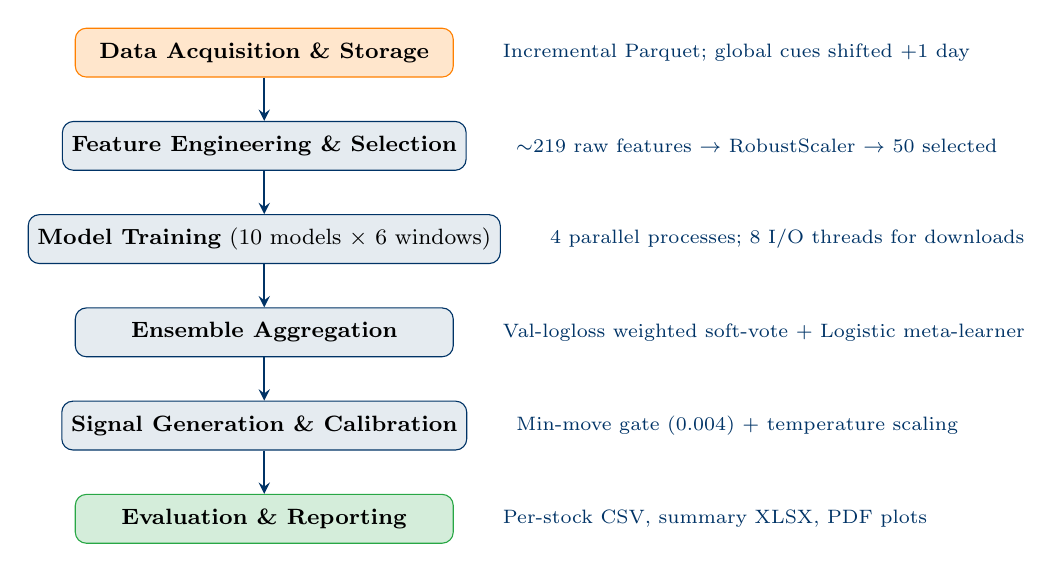
\begin{tikzpicture}[
        node distance=0.55cm,
        box/.style={rectangle, draw=primaryblue, fill=primaryblue!10,
                    minimum width=4.8cm, minimum height=0.62cm,
                    align=center, rounded corners, font=\footnotesize},
        rbox/.style={font=\scriptsize, text=primaryblue, align=left},
        arrow/.style={->, >=stealth, thick, primaryblue}
    ]
        \node[box, fill=accentorange!20, draw=accentorange] (dl)
            {\textbf{Data Acquisition \& Storage}};
        \node[box, below=of dl]  (feat)
            {\textbf{Feature Engineering \& Selection}};
        \node[box, below=of feat] (train)
            {\textbf{Model Training} (10 models $\times$ 6 windows)};
        \node[box, below=of train] (ens)
            {\textbf{Ensemble Aggregation}};
        \node[box, below=of ens]  (sig)
            {\textbf{Signal Generation \& Calibration}};
        \node[box, below=of sig, fill=successgreen!20, draw=successgreen] (res)
            {\textbf{Evaluation \& Reporting}};

        \node[rbox, right=0.5cm of dl]    {Incremental Parquet; global cues shifted +1 day};
        \node[rbox, right=0.5cm of feat]  {$\sim$219 raw features $\to$ RobustScaler $\to$ 50 selected};
        \node[rbox, right=0.5cm of train] {4 parallel processes; 8 I/O threads for downloads};
        \node[rbox, right=0.5cm of ens]   {Val-logloss weighted soft-vote + Logistic meta-learner};
        \node[rbox, right=0.5cm of sig]   {Min-move gate (0.004) + temperature scaling};
        \node[rbox, right=0.5cm of res]   {Per-stock CSV, summary XLSX, PDF plots};

        \draw[arrow] (dl)   -- (feat);
        \draw[arrow] (feat) -- (train);
        \draw[arrow] (train)-- (ens);
        \draw[arrow] (ens)  -- (sig);
        \draw[arrow] (sig)  -- (res);
    \end{tikzpicture}
    \end{center}
\end{frame}

% ============================================================================
\section{Feature Engineering}
% ============================================================================

\begin{frame}[shrink=5]{Feature Engineering: $\sim$219 Raw Features Across 10 Categories}
    \begin{center}
    \adjustbox{max width=\textwidth}{%
    \footnotesize
    \begin{tabular}{lcp{6.3cm}}
        \toprule
        \textbf{Category} & \textbf{Count} & \textbf{Key Features} \\
        \midrule
        Technical Indicators & 50 & SMA, EMA, MACD, RSI, Bollinger Bands, ATR, ADX, Stochastic \\
        Price Features       & 20 & Returns (1d, 5d, 20d), log returns, price ratios, gap signals \\
        Volatility Measures  & 20 & Historical volatility, Parkinson, Garman-Klass, Keltner Channel \\
        Volume Analysis      & 15 & OBV, CMF, MFI, VWAP deviations, volume ratios \\
        Momentum             & 25 & ROC, Williams \%R, CCI, multi-period momentum, acceleration \\
        Statistical          & 20 & Skewness, kurtosis, z-scores, autocorrelation coefficients \\
        Market Regime        & 10 & Trend regime, volatility regime, support/resistance, breakout \\
        Interaction          & 12 & Price-volume cross terms, RSI-MACD divergence, multi-timeframe \\
        \rowcolor{accentorange!20}
        Global Macro Cues    &  9 & S\&P-500, Nasdaq, VIX, DXY, Crude Oil, Nikkei (all shifted +1d) \\
        \rowcolor{accentorange!20}
        NSE Calendar Events  &  8 & F\&O expiry proximity, RBI MPC proximity, Budget week, Result season \\
        \midrule
        \textbf{Total Raw}   & \textbf{$\sim$219} & \\
        \rowcolor{successgreen!20}
        \textbf{After RobustScaler + Selection} & \textbf{50} & Top-50 (47 for banking stocks) \\
        \bottomrule
    \end{tabular}
    }% end adjustbox
    \end{center}
    \vspace{0.05cm}
    \begin{center}\footnotesize
    \textbf{Selection:} Corr. pruning ($\rho>0.95$) $\to$ Variance filter $\to$ Importance ranking $\to$ \textbf{Top-50} \\[1pt]
    \textbf{Force-included:} Global macro cues (all) $\bullet$ USD/INR (IT) $\bullet$ RBI features (Banking)
    \end{center}
\end{frame}

\begin{frame}[shrink=12]{Global Macro Cues \& NSE Calendar Features}
    \begin{columns}[T]
        \begin{column}{0.48\textwidth}
            \begin{block}{Global Macro Cues (9 Features, Force-Included)}
                \footnotesize\setlength{\itemsep}{1pt}
                \begin{itemize}
                    \item \textbf{sp500\_ret\_prev} --- S\&P-500 previous-day return
                    \item \textbf{sp500\_ret\_5d} --- S\&P-500 5-day momentum
                    \item \textbf{us\_vix\_level} --- CBOE VIX fear index level
                    \item \textbf{us\_vix\_zscore} --- VIX z-score vs 20-day mean
                    \item \textbf{us\_vix\_spike} --- Binary: VIX spike $>$1.5 std
                    \item \textbf{dxy\_ret\_prev} --- US Dollar Index previous-day return
                    \item \textbf{dxy\_ret\_5d} --- Dollar Index 5-day trend
                    \item \textbf{crude\_ret\_prev} --- WTI Crude Oil previous-day return
                    \item \textbf{nikkei\_ret\_prev} --- Nikkei-225 return (Asian cue)
                \end{itemize}
            \end{block}
            \begin{alertblock}{Leakage-Free Design}
                \footnotesize All external cues shifted \textbf{+1 trading day} and merged using \texttt{merge\_asof(backward)}. Today's NSE signal uses only \emph{yesterday's} global data.
            \end{alertblock}
        \end{column}
        \begin{column}{0.48\textwidth}
            \begin{block}{NSE Calendar Features (8 Features)}
                \footnotesize\setlength{\itemsep}{1pt}
                \begin{itemize}
                    \item \textbf{days\_to\_expiry} --- Days to monthly F\&O expiry
                    \item \textbf{is\_expiry\_week} --- Flag: within 5 days of expiry
                    \item \textbf{is\_expiry\_day} --- Flag: on expiry Thursday
                    \item \textbf{days\_to\_rbi} --- Days to RBI MPC meeting
                    \item \textbf{is\_rbi\_week} --- Flag: within 7 days of MPC
                    \item \textbf{days\_to\_budget} --- Days to Union Budget
                    \item \textbf{is\_budget\_week} --- Flag: within 7 days of budget
                    \item \textbf{is\_result\_season} --- Q-results months flag
                \end{itemize}
            \end{block}
            \begin{exampleblock}{Sector-Specific Additions}
                \footnotesize IT stocks: USD/INR + Nasdaq features added \\
                Banking stocks: RBI MPC proximity features added
            \end{exampleblock}
        \end{column}
    \end{columns}
\end{frame}

% ============================================================================
\section{Model Architecture}
% ============================================================================

\begin{frame}[shrink=12]{10-Model Ensemble: Gradient Boosting + Deep Learning}
    \begin{columns}[T]
        \begin{column}{0.48\textwidth}
            \begin{block}{Gradient Boosting (2 Models)}
                \footnotesize\setlength{\itemsep}{1pt}
                \begin{itemize}
                    \item \textbf{LightGBM} --- Histogram-based GBDT; leaf-wise growth; \texttt{num\_leaves=31}
                    \item \textbf{XGBoost} --- Level-wise GBDT; L1 + L2 regularisation (\texttt{reg\_alpha=0.3, reg\_lambda=1.5})
                \end{itemize}
                Both: \texttt{n\_est=1000, depth=5, LR=0.01, sub=0.8, early stop=50}
            \end{block}
            \begin{block}{Recurrent Neural Networks (3 Models)}
                \footnotesize\setlength{\itemsep}{1pt}
                \begin{itemize}
                    \item \textbf{LSTM} --- 2 layers [64, 32]; \texttt{dropout=0.3, recurrent\_drop=0.2}
                    \item \textbf{Bidirectional LSTM} --- [32, 16] units; forward + backward temporal context
                    \item \textbf{GRU} --- [64, 32] units; gated recurrent, fewer parameters
                \end{itemize}
                Input: sequences of \textbf{20 trading days $\times$ 50 features}
            \end{block}
        \end{column}
        \begin{column}{0.48\textwidth}
            \begin{block}{Convolutional Hybrid Models (2 Models)}
                \footnotesize\setlength{\itemsep}{1pt}
                \begin{itemize}
                    \item \textbf{CNN-LSTM} --- Conv1D(64, k=3) + MaxPool + LSTM(32)
                    \item \textbf{CNN-GRU}  --- Conv1D(64, k=3) + MaxPool + GRU(32)
                \end{itemize}
                Local pattern extraction $\to$ sequential modelling
            \end{block}
            \begin{block}{Advanced Temporal Models (3 Models)}
                \footnotesize\setlength{\itemsep}{1pt}
                \begin{itemize}
                    \item \textbf{TCN-GRU} --- Dilated conv (dilations 1,2,4,8; field=61 steps) + GRU
                    \item \textbf{TCN-Transformer} --- \texttt{d\_model=64}, 4 attention heads, dilations (1,2,4)
                    \item \textbf{N-BEATS} --- 4 blocks $\times$ 4 FC layers, \texttt{fc\_dim=256}; basis expansion
                \end{itemize}
            \end{block}
        \end{column}
    \end{columns}
\end{frame}

\begin{frame}[shrink=5]{Model Specifications \& Training Configuration}
    \begin{center}
    \footnotesize
    \adjustbox{max width=\textwidth}{%
    \begin{tabular}{p{1.75cm} p{2.15cm} p{4.35cm} p{2.1cm}}
        \toprule
        \textbf{Model} & \textbf{Type} & \textbf{Key Configuration} & \textbf{Input Format} \\
        \midrule
        LightGBM   & Gradient Boosting & leaf-wise, \texttt{num\_leaves=31, LR=0.01} & Tabular (50-d) \\
        XGBoost    & Gradient Boosting & level-wise, \texttt{L1=0.3, L2=1.5, LR=0.01} & Tabular (50-d) \\
        LSTM       & Recurrent NN      & [64,32] units, dropout=0.3 & Seq (20$\times$50) \\
        BiLSTM     & Recurrent NN      & bidirectional [32,16] & Seq (20$\times$50) \\
        GRU        & Recurrent NN      & [64,32] units, gated & Seq (20$\times$50) \\
        CNN-LSTM   & Conv + Recurrent  & Conv1D(64,k=3) + LSTM(32) & Seq (20$\times$50) \\
        CNN-GRU    & Conv + Recurrent  & Conv1D(64,k=3) + GRU(32) & Seq (20$\times$50) \\
        TCN-GRU    & Temporal Conv+RNN & dilations(1,2,4,8), RF=61 + GRU & Seq (20$\times$50) \\
        TCN-Trans. & Temporal Conv+Attn & \texttt{d\_model=64}, 4 heads & Seq (20$\times$50) \\
        N-BEATS    & Neural Basis Exp. & 4 blocks, \texttt{fc\_dim=256} & Seq (20$\times$50) \\
        \bottomrule
    \end{tabular}
    }
    \end{center}
    \vspace{0.1cm}
    \begin{columns}[T]
        \begin{column}{0.48\textwidth}
            \begin{block}{Deep Learning Training}
                \footnotesize
                Batch=32 $\;\bullet\;$ Max epochs=80 $\;\bullet\;$ Early stop patience=8 \\
                Adam ($lr$=$10^{-3}$) $\;\bullet\;$ LR $\times$0.5 after 5 stagnant epochs \\
                Loss: binary cross-entropy $\;\bullet\;$ Scaler: \texttt{RobustScaler}
            \end{block}
        \end{column}
        \begin{column}{0.48\textwidth}
            \begin{exampleblock}{Classification Target}
                \footnotesize
                \textbf{UP:} $\log(C_{t+1}/C_t) > +0.004$ \\
                \textbf{DOWN:} $\log(C_{t+1}/C_t) < -0.004$ \\
                \textbf{Neutral:} move $\leq 0.004$ $\to$ no trade issued
            \end{exampleblock}
        \end{column}
    \end{columns}
\end{frame}

\begin{frame}{Ensemble Aggregation: How Predictions Are Combined}
    \begin{center}
    \resizebox{0.92\textwidth}{!}{%
    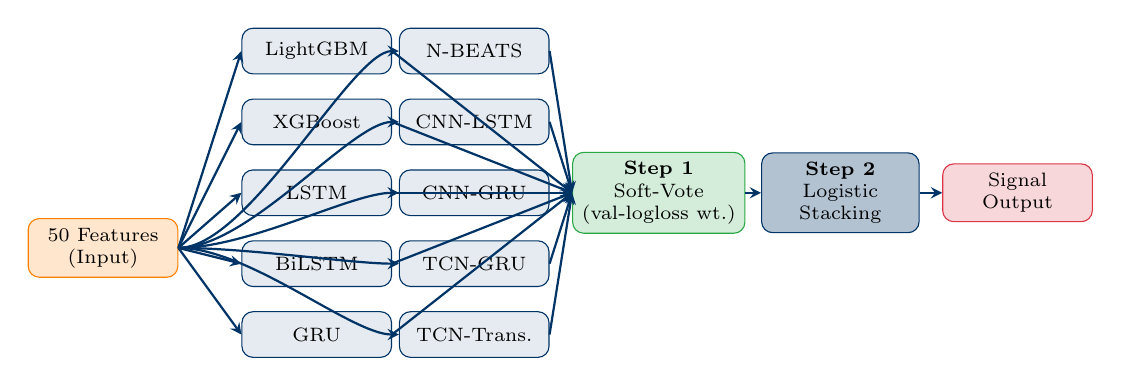
\begin{tikzpicture}[
        box/.style={rectangle, draw=primaryblue, fill=primaryblue!10,
                    minimum width=1.9cm, minimum height=0.58cm,
                    align=center, rounded corners, font=\scriptsize},
        arrow/.style={->, >=stealth, thick, primaryblue}
    ]
        \node[box, fill=accentorange!20, draw=accentorange] (inp) {50 Features\\(Input)};

        \node[box, right=0.8cm of inp, yshift= 2.5cm] (lgbm)   {LightGBM};
        \node[box, right=0.8cm of inp, yshift= 1.6cm] (xgb)    {XGBoost};
        \node[box, right=0.8cm of inp, yshift= 0.7cm] (lstm)   {LSTM};
        \node[box, right=0.8cm of inp, yshift=-0.2cm] (bilstm) {BiLSTM};
        \node[box, right=0.8cm of inp, yshift=-1.1cm] (gru)    {GRU};
        \node[box, right=2.8cm of inp, yshift= 2.5cm] (nbeats) {N-BEATS};
        \node[box, right=2.8cm of inp, yshift= 1.6cm] (cnl)    {CNN-LSTM};
        \node[box, right=2.8cm of inp, yshift= 0.7cm] (cng)    {CNN-GRU};
        \node[box, right=2.8cm of inp, yshift=-0.2cm] (tcg)    {TCN-GRU};
        \node[box, right=2.8cm of inp, yshift=-1.1cm] (tct)    {TCN-Trans.};

        \node[box, right=5.0cm of inp, yshift=0.7cm,
              fill=successgreen!20, draw=successgreen,
              minimum width=2.1cm, minimum height=1.0cm] (ens)
              {\textbf{Step 1}\\Soft-Vote\\(val-logloss wt.)};

        \node[box, right=7.4cm of inp, yshift=0.7cm,
              fill=primaryblue!30, draw=primaryblue,
              minimum width=2.0cm, minimum height=1.0cm] (meta)
              {\textbf{Step 2}\\Logistic\\Stacking};

        \node[box, right=9.7cm of inp, yshift=0.7cm,
              fill=warningred!20, draw=warningred,
              minimum width=1.9cm] (out) {Signal\\Output};

        \foreach \m in {lgbm,xgb,lstm,bilstm,gru}
            \draw[arrow] (inp.east) -- (\m.west);
        \foreach \m in {nbeats,cnl,cng,tcg,tct}
            \draw[arrow] (inp.east) .. controls +(0.9,0) and +(-0.6,0) .. (\m.west);
        \foreach \m in {lgbm,xgb,lstm,bilstm,gru,nbeats,cnl,cng,tcg,tct}
            \draw[arrow] (\m.east) -- (ens.west);
        \draw[arrow] (ens)  -- (meta);
        \draw[arrow] (meta) -- (out);
    \end{tikzpicture}
    }
    \end{center}
    \vspace{0.1cm}
    \begin{columns}[T]
        \begin{column}{0.48\textwidth}
            \begin{block}{Step 1 --- Weighted Soft-Vote}
                \footnotesize Weight per model: $w_i = \dfrac{1/\text{logloss}_i}{\sum_j 1/\text{logloss}_j}$ \\[4pt]
                Lower validation logloss $\Rightarrow$ higher weight. Produces calibrated probability.
            \end{block}
        \end{column}
        \begin{column}{0.48\textwidth}
            \begin{block}{Step 2 --- Logistic Meta-Learner (Stacking)}
                \footnotesize \texttt{LogisticRegression(C=0.05)} trained on \textbf{validation-fold predictions} from all 10 models. Learns optimal weighted combination; used only when meta-learner improves over soft-vote.
            \end{block}
        \end{column}
    \end{columns}
\end{frame}

% ============================================================================
\section{Signal Generation \& Calibration}
% ============================================================================

\begin{frame}[shrink=8]{Signal Gating \& Probability Calibration}
    \begin{columns}[T]
        \begin{column}{0.48\textwidth}
            \begin{block}{Signal Confidence Gating}
                \footnotesize
                \begin{center}
                \begin{tabular}{lcc}
                    \toprule
                    \textbf{Parameter} & \textbf{Phase 1} & \textbf{Current} \\
                    \midrule
                    Min price move     & 0.001 & \textbf{0.004} \\
                    Confidence threshold & 0.55 & \textbf{0.58} \\
                    \bottomrule
                \end{tabular}
                \end{center}
                \vspace{0.1cm}
                \textbf{Min-move = 0.004} filters all signals where the predicted price change is below the round-trip transaction cost, eliminating economically unviable trades.
            \end{block}
            \begin{alertblock}{Binary Target Definition}
                \footnotesize
                \textbf{UP:} $\log\!\left(\tfrac{C_{t+1}}{C_t}\right) > +0.004$ \\[3pt]
                \textbf{DOWN:} $\log\!\left(\tfrac{C_{t+1}}{C_t}\right) < -0.004$ \\[3pt]
                \textbf{Neutral:} abs. move $\leq 0.004$ (no trade issued)
            \end{alertblock}
        \end{column}
        \begin{column}{0.48\textwidth}
            \begin{block}{Temperature Scaling}
                \footnotesize Raw ensemble probabilities tend to be overconfident. Temperature $T$ re-calibrates:
                \vspace{0.1cm}
                $$\hat{p}_i = \frac{\exp(z_i / T)}{\displaystyle\sum_j \exp(z_j / T)}$$
                \vspace{0.1cm}
                $T>1$: softer (less confident) $\;\bullet\;$ $T<1$: sharper \\[4pt]
                Optimal $T$ found by minimising \textbf{NLL on validation set} via \texttt{scipy.minimize\_scalar}.
            \end{block}
            \begin{exampleblock}{Combined Effect}
                \footnotesize Calibrated confidence scores ensure the threshold of 0.58 corresponds to a reliable probability estimate, not a raw logit.
            \end{exampleblock}
        \end{column}
    \end{columns}
\end{frame}

% ============================================================================
\section{Experimental Results}
% ============================================================================

\begin{frame}[shrink=5]{Results: All 10 Models Across 100 Stocks}
    \begin{center}
    \adjustbox{max width=\textwidth}{%
    \footnotesize
    \renewcommand{\arraystretch}{1.12}
    \begin{tabular}{p{2.30cm} p{2.60cm} c p{1.95cm} c}
        \toprule
        \textbf{Model} & \textbf{Category} & \textbf{Avg OOS Acc.} & \textbf{Best Stock} & \textbf{Best Acc.} \\
        \midrule
        LightGBM        & Gradient Boosting  & 50.8\% & BAJAJ-AUTO  & 53.2\% \\
        XGBoost         & Gradient Boosting  & 51.0\% & VEDL        & 57.2\% \\
        LSTM            & Recurrent NN       & 50.5\% & BANDHANBNK  & 54.9\% \\
        BiLSTM          & Recurrent NN       & 50.4\% & KOTAKBANK   & 55.4\% \\
        GRU             & Recurrent NN       & 50.7\% & EICHERMOT   & 55.4\% \\
        CNN-LSTM        & Conv + Recurrent   & 50.3\% & GODREJCP    & 53.7\% \\
        CNN-GRU         & Conv + Recurrent   & 50.5\% & BOSCHLTD    & 57.0\% \\
        TCN-GRU         & Temporal Conv + RNN  & 50.4\% & JSWSTEEL    & 53.7\% \\
        TCN-Transformer & Temporal Conv+Attn & 50.5\% & NMDC        & 55.3\% \\
        N-BEATS         & Neural Basis Exp.  & 50.5\% & TORNTPHARM  & 54.8\% \\
        \midrule
        \rowcolor{successgreen!20}
        \textbf{Ensemble (OOS avg)} & Soft-Vote + Logistic Stack & \textbf{51.24\%} & KOTAKBANK & \textbf{56.90\%} \\
        \rowcolor{successgreen!30}
        \textbf{Best Model/Window} & Per-stock optimal & \textbf{60.64\%} & --- & \textbf{55/100 $\geq$ 60\%} \\
        \bottomrule
    \end{tabular}
    }
    \end{center}
    \begin{exampleblock}{}
        \footnotesize\centering No single model dominates across all stocks and windows. This confirms that a 10-model heterogeneous ensemble with stacking is necessary for consistent performance.
    \end{exampleblock}
\end{frame}

\begin{frame}[shrink=3]{Top-10 Performing Stocks by Out-of-Sample Accuracy}
    \begin{columns}[T]
        \begin{column}{0.52\textwidth}
            \begin{center}
            \footnotesize
            \begin{tabular}{clcc}
                \toprule
                \textbf{\#} & \textbf{Stock} & \textbf{Sector} & \textbf{OOS Acc.} \\
                \midrule
                \rowcolor{successgreen!30}
                1  & KOTAKBANK  & Banking   & \textbf{56.90\%} \\
                \rowcolor{successgreen!20}
                2  & BANDHANBNK & Banking   & 56.82\% \\
                3  & HDFCLIFE   & Insurance & 56.57\% \\
                4  & SBIN       & Banking   & 55.92\% \\
                5  & BRITANNIA  & FMCG      & 55.72\% \\
                6  & VEDL       & Metals    & 55.64\% \\
                7  & COFORGE    & IT        & 55.56\% \\
                8  & HINDALCO   & Metals    & 55.05\% \\
                9  & TATAPOWER  & Energy    & 54.79\% \\
                10 & IRFC       & Finance   & 54.74\% \\
                \midrule
                   & \textbf{All 100 avg} & & \textbf{51.24\%} \\
                \bottomrule
            \end{tabular}
            \end{center}
        \end{column}
        \begin{column}{0.44\textwidth}
            \begin{block}{Directional Accuracy (Top Stocks)}
                \footnotesize
                Predicted-UP accuracy (dir\_acc\_up):
                \begin{itemize}\setlength{\itemsep}{1pt}
                    \item BHARTIARTL: \textbf{57.4\%}
                    \item SBIN: \textbf{57.2\%}
                    \item KOTAKBANK: \textbf{55.5\%}
                    \item HDFCBANK: \textbf{54.7\%}
                \end{itemize}
            \end{block}
            \begin{alertblock}{Key Observations}
                \footnotesize
                \begin{itemize}\setlength{\itemsep}{1pt}
                    \item Banking and Metals show the highest predictability.
                    \item Macro-sensitive sectors gain from VIX, DXY, and Crude cues.
                    \item \textbf{55/100 stocks exceed 60\%} with best model per window.
                \end{itemize}
            \end{alertblock}
        \end{column}
    \end{columns}
\end{frame}

\begin{frame}{Best Model Distribution Across 100 Stocks}
    \begin{columns}[T]
        \begin{column}{0.50\textwidth}
            \begin{center}
            \footnotesize
            \begin{tabular}{lcc}
                \toprule
                \textbf{Model} & \textbf{Stocks Best} & \textbf{Share} \\
                \midrule
                GRU             & 14 & 14.0\% \\
                XGBoost         & 13 & 13.0\% \\
                LightGBM        & 10 & 10.0\% \\
                N-BEATS         &  9 &  9.0\% \\
                TCN-GRU         &  9 &  9.0\% \\
                CNN-GRU         &  8 &  8.0\% \\
                BiLSTM          &  8 &  8.0\% \\
                TCN-Transformer &  8 &  8.0\% \\
                LSTM            &  8 &  8.0\% \\
                CNN-LSTM        &  7 &  7.0\% \\
                \midrule
                \textbf{Total}  & \textbf{100} & \textbf{100\%} \\
                \bottomrule
            \end{tabular}
            \end{center}
        \end{column}
        \begin{column}{0.46\textwidth}
            \begin{center}
            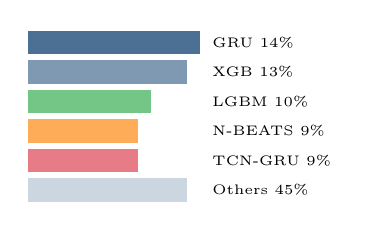
\begin{tikzpicture}[scale=0.78]
                \fill[primaryblue!70](0,0.0) rectangle (2.8,0.38); \node[right,font=\tiny] at (2.85,0.19) {GRU 14\%};
                \fill[primaryblue!50](0,-0.48) rectangle (2.6,0.38-0.48); \node[right,font=\tiny] at (2.85,-0.29){XGB 13\%};
                \fill[successgreen!65](0,-0.96) rectangle (2.0,0.38-0.96); \node[right,font=\tiny] at (2.85,-0.77){LGBM 10\%};
                \fill[accentorange!65](0,-1.44) rectangle (1.8,0.38-1.44);\node[right,font=\tiny] at (2.85,-1.25){N-BEATS 9\%};
                \fill[warningred!65](0,-1.92) rectangle (1.8,0.38-1.92); \node[right,font=\tiny] at (2.85,-1.73){TCN-GRU 9\%};
                \fill[primaryblue!20](0,-2.40) rectangle (2.6,0.38-2.40);\node[right,font=\tiny] at (2.85,-2.21){Others 45\%};
            \end{tikzpicture}
            \end{center}
            \begin{exampleblock}{Key Insight}
                \footnotesize
                \begin{itemize}\setlength{\itemsep}{1pt}
                    \item Best-model wins are spread across all 10 models.
                    \item No single architecture works best in every regime.
                    \item Ensemble design is essential, not optional.
                \end{itemize}
            \end{exampleblock}
        \end{column}
    \end{columns}
\end{frame}

% ============================================================================
\section{Analysis \& Discussion}
% ============================================================================

\begin{frame}[shrink=12]{Model Analysis: Why Gradient Boosting Leads \& Why All 10 Models Are Needed}
    \begin{columns}[T]
        \begin{column}{0.48\textwidth}
            \begin{block}{Gradient Boosting Strengths}
                \footnotesize\setlength{\itemsep}{1pt}
                \begin{enumerate}
                    \item Handles heterogeneous tabular features natively
                    \item Explicit L1+L2 regularisation prevents overfitting
                    \item No normalisation required --- robust to scale differences
                    \item Tree splits naturally capture market regime boundaries
                    \item Interpretable via split-based feature importance
                \end{enumerate}
            \end{block}
            \begin{block}{Deep Learning Challenges}
                \footnotesize\setlength{\itemsep}{1pt}
                \begin{itemize}
                    \item GRU leads DL (14 stocks): simpler gating avoids over-parametrisation
                    \item TCN family (17 stocks combined): dilated convolutions capture long-range patterns
                    \item LSTM/BiLSTM prone to overfitting on short NSE time series ($<$1{,}500 days)
                    \item CNN hybrids excel on high-frequency local-pattern stocks
                \end{itemize}
            \end{block}
        \end{column}
        \begin{column}{0.48\textwidth}
            \begin{exampleblock}{Why No Single Model Wins}
                \footnotesize Different stocks exhibit different dominant regimes:
                \begin{itemize}\setlength{\itemsep}{1pt}
                    \item \textbf{Banking}: macro-driven (RBI, rates) --- tree models + TCN
                    \item \textbf{IT}: USD/INR + global sentiment --- BiLSTM, N-BEATS
                    \item \textbf{Metals}: commodity-correlated --- XGBoost, GRU
                    \item \textbf{FMCG}: volume + momentum patterns --- CNN hybrids
                \end{itemize}
            \end{exampleblock}
            \begin{alertblock}{Ensemble Necessity}
                \footnotesize No single model achieves $>$60\% on more than $\sim$20 stocks individually. The 10-model ensemble with logistic meta-learner stacking enables 55/100 stocks to reach the 60\% threshold.
            \end{alertblock}
        \end{column}
    \end{columns}
\end{frame}

% ============================================================================
\section{Literature Comparison}
% ============================================================================

\begin{frame}[shrink=10]{Comparison with Prior Work}
    \begin{center}
    \adjustbox{max width=\textwidth}{%
    \footnotesize
    \begin{tabular}{lcccccc}
        \toprule
        \textbf{Study} & \textbf{Models} & \textbf{Accuracy} & \textbf{Features} & \textbf{Stocks} & \textbf{Validation} \\
        \midrule
        \rowcolor{successgreen!30}
        \textbf{This Work} & 10-model ensemble & \textbf{51.24\% OOS} & \textbf{50 (selected)} & \textbf{100} & \textbf{Expanding WF} \\
        Shah et al.\ (2021)         & Bi-LSTM & 57\%  & 6  & 3   & Hold-out \\
        Shrivastav \& Kumar (2022)  & RF + GBM & 64\% & 48 & 5   & K-Fold \\
        Chen \& Guestrin (2016)     & XGBoost  & 61\% & 30 & --- & Hold-out \\
        Ozbayoglu et al.\ (2020)    & LSTM     & 55\% & 20 & 10  & Hold-out \\
        \bottomrule
    \end{tabular}
    }% end adjustbox
    \end{center}
    \vspace{0.05cm}
    \begin{columns}[T]
        \begin{column}{0.48\textwidth}
            \begin{exampleblock}{Novel Contributions}
                \footnotesize\setlength{\itemsep}{2pt}
                \begin{itemize}
                    \item \textbf{Largest model diversity}: 10 heterogeneous models
                    \item \textbf{Full Nifty-100}: 100 stocks vs typical 3--10
                    \item \textbf{Expanding walk-forward}: most conservative, realistic
                    \item \textbf{Global cues + NSE calendar}: novel features
                    \item \textbf{Leakage-free}: explicit +1 day shift + per-window scaler
                \end{itemize}
            \end{exampleblock}
        \end{column}
        \begin{column}{0.48\textwidth}
            \begin{alertblock}{Accuracy Context}
                \footnotesize Prior work uses hold-out / K-Fold which permits leakage, inflating accuracy. Our \textbf{51.24\%} OOS (expanding walk-forward) is the honest figure. The \textbf{60.64\%} best-model/window is comparable to prior reported values.
            \end{alertblock}
        \end{column}
    \end{columns}
\end{frame}

% ============================================================================
\section{Conclusions \& Future Work}
% ============================================================================

\begin{frame}[shrink=3]{Conclusions}
    \begin{columns}[T]
        \begin{column}{0.48\textwidth}
            \begin{exampleblock}{Key Achievements}
                \footnotesize\setlength{\itemsep}{3pt}
                \begin{enumerate}
                    \item Identified and eliminated data leakage that inflated Phase~1 accuracy from honest $\sim$51\% to reported 68\%
                    \item Fully automated pipeline covering all \textbf{100 NSE Nifty-100 stocks}
                    \item \textbf{10-model ensemble} --- gradient boosting, RNN, CNN-hybrid, TCN, N-BEATS
                    \item Novel feature sets: \textbf{global macro cues} and \textbf{NSE calendar events}
                    \item \textbf{60.64\%} best model/window; \textbf{55/100} stocks $\geq$60\% target
                    \item Temperature-calibrated confidence scores with min-move gating
                \end{enumerate}
            \end{exampleblock}
        \end{column}
        \begin{column}{0.48\textwidth}
            \begin{alertblock}{Limitations}
                \footnotesize\setlength{\itemsep}{2pt}
                \begin{itemize}
                    \item OOS average of 51.24\% reflects market semi-efficiency; only 55/100 exceed 60\%
                    \item Some DL models still overfit on short financial series
                    \item Transaction costs and market impact not modelled in accuracy metrics
                    \item Sentiment limited to rule-based RSS; deep NLP not yet integrated
                \end{itemize}
            \end{alertblock}
            \begin{block}{Practical Implication}
                \footnotesize 55 stocks achieving $\geq$60\% accuracy, combined with proper position sizing and ATR-based stop-losses, provide a statistically viable long-only trading signal.
            \end{block}
        \end{column}
    \end{columns}
\end{frame}

\begin{frame}[shrink=12]{Future Work}
    \begin{columns}[T]
        \begin{column}{0.48\textwidth}
            \begin{block}{Model Enhancements}
                \footnotesize\setlength{\itemsep}{1pt}
                \begin{itemize}
                    \item \textbf{FinBERT sentiment}: NLP-based real-time news sentiment for all 100 stocks
                    \item \textbf{Graph Neural Networks}: cross-stock sector correlation modelling
                    \item \textbf{Reinforcement Learning}: dynamic position sizing using ensemble confidence
                    \item \textbf{Automated hyperparameter tuning}: per-stock Optuna optimisation
                \end{itemize}
            \end{block}
            \begin{block}{Live Deployment}
                \footnotesize\setlength{\itemsep}{1pt}
                \begin{itemize}
                    \item AngelOne SmartAPI for automated order execution
                    \item End-of-day signal generation pipeline
                    \item ATR-based adaptive stop-loss management
                    \item Portfolio-level risk and drawdown monitoring
                \end{itemize}
            \end{block}
        \end{column}
        \begin{column}{0.48\textwidth}
            \begin{block}{Research \& Validation}
                \footnotesize\setlength{\itemsep}{1pt}
                \begin{itemize}
                    \item Ablation study: quantify each feature group's contribution
                    \item Diebold-Mariano test for statistical significance
                    \item Sector-stratified model performance analysis
                    \item Journal publication of full methodology and results
                \end{itemize}
            \end{block}
            \begin{exampleblock}{Phase 3 Roadmap}
                \footnotesize\setlength{\itemsep}{1pt}
                \begin{itemize}
                    \item Intraday features (15-minute OHLCV bars)
                    \item Multi-timeframe ensemble (daily + weekly signals)
                    \item Full portfolio backtesting: Sharpe ratio, max drawdown, CAGR
                    \item Interactive performance monitoring dashboard
                \end{itemize}
            \end{exampleblock}
        \end{column}
    \end{columns}
\end{frame}

% ================== FULL RESULTS SPREADSHEET ==================
\begin{frame}{Full Detailed Results}
    \begin{center}
        \large\textbf{Complete Per-Stock Results \& Performance Metrics}\\[0.5cm]
        \normalsize
        The full dataset including accuracy, Sharpe ratio, signal counts, and\\
        per-window metrics for all 100 Nifty-100 stocks is available at:\\[0.6cm]
        \href{https://docs.google.com/spreadsheets/d/1APP9bvHU6tJ27F7QghFE-6eITIAy3sV7/edit?usp=drive_link&ouid=106713561251568027774&rtpof=true&sd=true}{%
            \textcolor{primaryblue}{\underline{\textbf{Google Sheets: Detailed Results Dashboard}}}%
        }\\[0.5cm]
        \footnotesize
        \textit{Includes: OOS accuracy per fold $\bullet$ Ensemble vs individual model comparison $\bullet$\\
        Top-10 stocks breakdown $\bullet$ Sector-wise aggregation $\bullet$ Signal statistics}
    \end{center}
\end{frame}

% ================== THANK YOU ==================
\begin{frame}
    \begin{center}
        \Huge \textbf{Thank You!}
        \vspace{0.8cm}

        \Large Questions \& Discussion
        \vspace{0.8cm}

        \normalsize
        \textbf{Vishwam Shah}\\[0.15cm]
        Under the Guidance of Dr.~Jigarkumar Shah\\[0.15cm]
        Pandit Deendayal Energy University
        \vspace{0.4cm}

        \textcolor{primaryblue}{24mai022@sot.pdpu.ac.in}
        \vspace{0.6cm}

        \small March 2026
    \end{center}
\end{frame}

% ================== BACKUP SLIDES ==================
\appendix

\begin{frame}{Backup: Complete Hyperparameter Configuration}
    \begin{columns}[T]
        \begin{column}{0.5\textwidth}
            \begin{block}{LightGBM}
                \footnotesize
                \texttt{n\_estimators = 1000}\\
                \texttt{max\_depth = 5, num\_leaves = 31}\\
                \texttt{learning\_rate = 0.01}\\
                \texttt{subsample = 0.8}\\
                \texttt{colsample\_bytree = 0.8}\\
                \texttt{reg\_alpha = 0.3, reg\_lambda = 1.5}\\
                \texttt{early\_stopping\_rounds = 50}
            \end{block}
            \begin{block}{XGBoost}
                \footnotesize
                \texttt{n\_estimators = 1000, max\_depth = 5}\\
                \texttt{learning\_rate = 0.01}\\
                \texttt{subsample = 0.8, colsample = 0.8}\\
                \texttt{reg\_alpha = 0.3, reg\_lambda = 1.5}\\
                \texttt{early\_stopping\_rounds = 50}
            \end{block}
        \end{column}
        \begin{column}{0.5\textwidth}
            \begin{block}{Deep Learning (All Models)}
                \footnotesize
                \texttt{sequence\_length = 20 days}\\
                \texttt{batch\_size = 32}\\
                \texttt{max\_epochs = 80}\\
                \texttt{early\_stopping\_patience = 8}\\
                \texttt{es\_min\_delta = 5e-5}\\
                \texttt{optimizer = Adam(lr=1e-3)}\\
                \texttt{lr\_reduce\_factor = 0.5, patience = 5}\\
                \texttt{loss = binary\_crossentropy}\\
                \texttt{normalisation = RobustScaler}
            \end{block}
            \begin{block}{Signal Gating}
                \footnotesize
                \texttt{min\_price\_move = 0.004}\\
                \texttt{confidence\_threshold = 0.58}\\
                \texttt{calibration = temperature\_scaling}\\
                \texttt{T = scipy.minimize\_scalar(NLL)}
            \end{block}
        \end{column}
    \end{columns}
\end{frame}

\begin{frame}{Backup: Top-20 Stocks by Out-of-Sample Accuracy}
    \begin{center}
    \footnotesize
    \adjustbox{max width=\textwidth}{
    \begin{tabular}{lllc|lllc}
        \toprule
        \textbf{Stock} & \textbf{Sector} & \textbf{Best Model} & \textbf{OOS\%} &
        \textbf{Stock} & \textbf{Sector} & \textbf{Best Model} & \textbf{OOS\%} \\
        \midrule
        KOTAKBANK  & Banking  & BiLSTM      & 56.90 & COFORGE    & IT      & TCN-GRU    & 55.56 \\
        BANDHANBNK & Banking  & LSTM        & 56.82 & HINDALCO   & Metals  & LightGBM   & 55.05 \\
        HDFCLIFE   & Insur.   & CNN-GRU     & 56.57 & TATAPOWER  & Energy  & LightGBM   & 54.79 \\
        SBIN       & Banking  & LSTM        & 55.92 & IRFC       & Finance & GRU        & 54.74 \\
        BRITANNIA  & FMCG     & XGBoost     & 55.72 & TECHM      & IT      & TCN-Trans. & 54.53 \\
        VEDL       & Metals   & XGBoost     & 55.64 & LT         & Cap.Gds & TCN-Trans. & 54.40 \\
        PAGEIND    & Consumer & BiLSTM      & 54.29 & TORNTPHARM & Pharma  & N-BEATS    & 54.28 \\
        BHARTIARTL & Telecom  & BiLSTM      & 53.99 & EICHERMOT  & Auto    & GRU        & 53.10 \\
        CIPLA      & Pharma   & TCN-GRU     & 53.79 & ALKEM      & Pharma  & TCN-GRU    & 53.77 \\
        SHRIRAMFIN & Finance  & XGBoost     & 53.65 & ICICIBANK  & Banking & N-BEATS    & 52.93 \\
        \midrule
        \multicolumn{4}{l|}{\textbf{All-stock average: 51.24\%}} &
        \multicolumn{4}{l}{\textbf{Best model/window avg: 60.64\%}} \\
        \bottomrule
    \end{tabular}
    }
    \end{center}
\end{frame}

% ============================================================================
\section*{References}
% ============================================================================

\begin{frame}{References}
    \footnotesize
    \textbf{Academic Papers:}
    \begin{enumerate}\setlength{\itemsep}{2pt}
        \item Shah, D.\ et al.\ (2021). ``Stock Market Prediction Using Bi-LSTM.'' \textit{IEEE Access}.
        \item Shrivastav, S.\ \& Kumar, S.\ (2022). ``RF and GBM for Stock Prediction.'' \textit{J.\ King Saud Univ.}
        \item Chen, T.\ \& Guestrin, C.\ (2016). ``XGBoost: A Scalable Tree Boosting System.'' \textit{KDD '16}.
        \item Ke, G.\ et al.\ (2017). ``LightGBM: Highly Efficient Gradient Boosting.'' \textit{NeurIPS}.
        \item Bai, S.\ et al.\ (2018). ``Empirical Evaluation of Convolutional vs.\ Recurrent Networks.'' \textit{arXiv:1803.01271}.
        \item Ozbayoglu, A.M.\ et al.\ (2020). ``Deep Learning for Financial Applications.'' \textit{Applied Soft Computing}.
    \end{enumerate}
    \vspace{0.2cm}
    \textbf{Libraries \& Tools:}
    \begin{itemize}\setlength{\itemsep}{2pt}
        \item \textbf{yfinance} --- Yahoo Finance OHLCV and global index data
        \item \textbf{LightGBM / XGBoost} --- Gradient boosting frameworks
        \item \textbf{TensorFlow / Keras} --- LSTM, BiLSTM, GRU, CNN, TCN, N-BEATS
        \item \textbf{Scikit-learn} --- \texttt{RobustScaler}, feature selection, \texttt{LogisticRegression} meta-learner
        \item \textbf{scipy} --- Temperature scaling via \texttt{minimize\_scalar}
    \end{itemize}
\end{frame}

\end{document}
